\documentclass{article}
\usepackage{amsmath}
\usepackage{amsfonts}
\usepackage{hyperref}
\usepackage{graphicx}
\usepackage{tikz}
\usetikzlibrary{positioning, automata}
\usepackage{setspace}
\usepackage{fancyhdr}
\usepackage{float}
\usepackage[a4paper, margin=1in]{geometry}


\newcommand{\R}{\mathbb{R}}

\pagestyle{fancy}
\begin{document}


\author{kipngeno koech - bkoech}
\title{Homework 4 - Applied Stochastic Processes}   
\maketitle

\medskip

\section*{Question 1: MoM, MLE, Bias and Consistency (20 points)}

Consider a normal distribution defined by the probability density function (PDF):

\[
f(y; \mu, \sigma) = \frac{1}{\sqrt{2\pi\sigma^2}} e^{-\frac{(y - \mu)^2}{2\sigma^2}}, \quad -\infty < y < \infty,
\]

\noindent where \(\mu\) is the mean and \(\sigma^2\) is the variance. Given a random sample \(Y = \{ y_1, y_2, \ldots, y_n \}\) drawn from this normal distribution, perform the following tasks:

\begin{enumerate}
    \item[(a)] \textbf{(5 points)} Use the method of moments to derive the estimators for \(\mu\) and \(\sigma^2\).
    \[
    \hat{\mu}_{\text{MoM}} = \frac{1}{n} \sum_{i=1}^{n} y_i, \quad \hat{\sigma}^2_{\text{MoM}} = \frac{1}{n} \sum_{i=1}^{n} (y_i - \hat{\mu}_{\text{MoM}})^2.
    \]

     \item[(b)] \textbf{(5 points)} Derive the Maximum Likelihood Estimators (MLE) for \(\mu\) and \(\sigma^2\).

     \item[(c)] \textbf{(3 points)} Calculate the bias of the MoM estimators \(\hat{\mu}_{\text{MoM}}\) and \(\hat{\sigma}^2_{\text{MoM}}\).
     
    \item[(d)] \textbf{(3 points)} Calculate the bias of the MLE estimators \(\hat{\mu}_{\text{MLE}}\) and \(\hat{\sigma}^2_{\text{MLE}}\).

    \item[(e)] \textbf{(4 points)} Show that both the MoM and MLE estimators are consistent, meaning that as \(n \to \infty\), \(\hat{\mu}_{\text{MoM}} \to \mu\), \(\hat{\sigma}^2_{\text{MoM}} \to \sigma^2\), \(\hat{\mu}_{\text{MLE}} \to \mu\), and \(\hat{\sigma}^2_{\text{MLE}} \to \sigma^2\) in probability.
\end{enumerate}
    
  








\section*{Question 2: Spam-Ham Detection Using MLE and MAP (30 points)}
In digital communication, distinguishing spam from ham (non-spam) is crucial for email security. Statistical techniques such as Maximum Likelihood Estimation (MLE) and Maximum A Posteriori (MAP) estimation are effective for classification. This section aims to build a spam-ham classifier using both MLE and MAP methods.

\subsection*{Part 1: MLE/MAP on Toy Dataset (10 points)}
You are provided with a mini dataset containing six SMS messages labeled as either spam or ham. A single feature, ``offer,'' indicates the presence (1) or absence (0) of the word ``offer'' in each message.

\begin{table}[h!]
    \centering
    \begin{tabular}{|c|l|c|c|}
        \hline
        \textbf{Message ID} & \textbf{Message Content} & \textbf{``Offer'' (X)} & \textbf{Class (Y)} \\
        \hline
        1 & ``Special offer now!'' & 1 & 1 (Spam) \\
        2 & ``Meeting at 10 AM'' & 0 & 0 (Ham) \\
        3 & ``Claim your offer'' & 1 & 1 (Spam) \\
        4 & ``Lunch tomorrow?'' & 0 & 0 (Ham) \\
        5 & ``Free offer available!'' & 1 & 1 (Spam) \\
        6 & ``Hello, how are you?'' & 0 & 0 (Ham) \\
        \hline
    \end{tabular}
    \caption{Mini Dataset for Spam-Ham Detection}
\end{table}

\noindent Calculate the following MLE estimates:
\begin{itemize}
    \item[(a)] \textbf{(1 point)} $\pi = P(Y = 1)$: Probability that a message is spam.
    \[
    \hat{\pi}_{\text{MLE}} = \frac{\text{Number of spam messages}}{\text{Total number of messages}} = \frac{3}{6} = \mathbf{\frac{1}{2}}
    \]
    \item[(b)] \textbf{(1 point)} $\theta_{\text{spam}} = P(X = 1 \mid Y = 1)$: Probability that ``offer'' appears in a spam message.
    \[
    \hat{\theta}_{\text{spam}} = \frac{\text{Number of spam messages with ``offer''}}{\text{Total number of spam messages}} = \frac{3}{3} = \mathbf{1}
    \]
    \item[(c)] \textbf{(1 point)} $\theta_{\text{ham}} = P(X = 1 \mid Y = 0)$: Probability that ``offer'' appears in a ham message.
    \[
    \hat{\theta}_{\text{ham}} = \frac{\text{Number of ham messages with ``offer''}}{\text{Total number of ham messages}} = \frac{0}{3} = \mathbf{0}
    \]
    \item[(d)] \textbf{(2 points)} Derive the likelihood function and maximize it to find the parameter estimates. 
    \[
    \hat{\pi}_{\text{MLE}} = \frac{3}{6} = \mathbf{\frac{1}{2}}, \quad \hat{\theta}_{\text{spam}} = 1, \quad \hat{\theta}_{\text{ham}} = 0
    \]
\end{itemize}

\noindent Assume Beta priors:
\begin{itemize}
    \item[(e)] \textbf{(2 points)} $\pi \sim \text{Beta}(2, 2)$
    \[
    P(\pi) = \frac{1}{B(2, 2)} \pi^{2-1} (1 - \pi)^{2-1} = 6\pi(1 - \pi)
    \]
    \[
    P(\pi \mid \text{data}) \propto P(\text{data} \mid \pi) P(\pi) = \pi^3 (1 - \pi)^3
    \]
    \[
    \hat{\pi}_{\text{MAP}} = \frac{3}{6} = \mathbf{\frac{1}{2}}
    \]
    \item[(f)] \textbf{(2 points)} $\theta_{\text{spam}} \sim \text{Beta}(2, 1)$
    \[
    P(\theta_{\text{spam}}) = \frac{1}{B(2, 1)} \theta_{\text{spam}}^{2-1} (1 - \theta_{\text{spam}})^{1-1} = 2\theta_{\text{spam}}
    \]
    \[
    P(\theta_{\text{spam}} \mid \text{data}) \propto P(\text{data} \mid \theta_{\text{spam}}) P(\theta_{\text{spam}}) = \theta_{\text{spam}}^3 (1 - \theta_{\text{spam}})
    \]
    \[
    \hat{\theta}_{\text{spam, MAP}} = \frac{3}{3} = \mathbf{1}
    \]
    \item[(g)] \textbf{(2 points)} $\theta_{\text{ham}} \sim \text{Beta}(1, 2)$
    \[
    P(\theta_{\text{ham}}) = \frac{1}{B(1, 2)} \theta_{\text{ham}}^{1-1} (1 - \theta_{\text{ham}})^{2-1} = 2(1 - \theta_{\text{ham}})
    \]
    \[
    P(\theta_{\text{ham}} \mid \text{data}) \propto P(\text{data} \mid \theta_{\text{ham}}) P(\theta_{\text{ham}}) = (1 - \theta_{\text{ham}})^3
    \]
    \[
    \hat{\theta}_{\text{ham, MAP}} = \frac{0}{3} = \mathbf{0}
    \]
\end{itemize}

\noindent Calculate the MAP estimates for $\pi$, $\theta_{\text{spam}}$, and $\theta_{\text{ham}}$ using prior information. 


\subsection*{Part 2: Practical Implications (4 points)}
Discuss the following:
\begin{enumerate}
    \item[(a)] \textbf{(1 point)} How do different prior choices affect MAP estimates?
    \\\\ A prior that aligns with the true underlying distribution can lead to more accurate estimates, while a less informative prior may introduce bias or uncertainty in the estimates.
    \item[(b)] \textbf{(1 point)} Why might MLE overfit with small datasets?
    \\\\ MLE tends to overfit with small datasets because it maximizes the likelihood of the observed data, which can lead to high variance and poor generalization to new data.
    \item[(c)] \textbf{(1 point)} In what scenarios would MLE or MAP perform better?
    \\\\ MLE is preferred when prior information is limited or unnecessary, while MAP is beneficial when incorporating prior knowledge can improve estimation accuracy.
    \item[(d)] \textbf{(1 point)} What is the bias-variance trade-off between MLE and MAP?
    \\\\ MLE tends to have lower bias but higher variance, while MAP can introduce bias but reduce variance by incorporating prior information.
\end{enumerate}

\subsection*{Part 3: Real-World Implementation (10 points)}
In this exercise, you will classify messages as either "spam" or "ham" (not spam) using a Naive Bayes classifier. You will implement two different estimation methods. Use the ``SMS Spam Collection'' dataset, available at \href{https://archive.ics.uci.edu/ml/datasets/SMS+Spam+Collection}{this link}, to implement a spam-ham detection classifier using:

\begin{itemize}
    \item \textbf{Maximum Likelihood Estimation (MLE)}: Estimates the parameters based solely on the training data without prior beliefs about the parameters.
    \item \textbf{Maximum A Posteriori (MAP)}: Incorporates prior beliefs about the parameters into the estimation, using Laplace smoothing to handle zero probabilities.
\end{itemize}

"

\subsection*{Tasks}

\subsubsection*{Step 1: Data Loading and Preprocessing}
\begin{enumerate}
    \item \textbf{Load the Dataset}:
    \begin{itemize}
        \item Download the SMS Spam Collection dataset and load it into your environment using pandas.
        \item Ensure the dataset is read correctly, with columns labeled "label" for spam/ham and "message" for the text content.
    \end{itemize}
    
    \item \textbf{Preprocess the Text Messages}:
    \begin{itemize}
        \item Convert all text to lowercase.
        \item Remove punctuation and special characters.
        \item Tokenize the messages (split the messages into words).
    \end{itemize}
    Example Preprocessing Steps:
    \begin{itemize}
        \item Lowercasing: Convert ``Hello!'' to ``hello''.
        \item Remove punctuation: Convert ``This is spam!!!'' to ``this is spam''.
    \end{itemize}
    
    \item \textbf{Split the Dataset}:
    \begin{itemize}
        \item Divide the dataset into training and test sets (e.g., 80\% training, 20\% testing).
        \item Ensure that both sets maintain the same class distribution.
    \end{itemize}
\end{enumerate}

\subsubsection*{Step 2: Implement Maximum Likelihood Estimator (MLE)}
\begin{enumerate}
    \item \textbf{Calculate Probabilities}:
    \begin{itemize}
        \item For each class (spam and ham), calculate the probability of each word appearing in that class based on the training data.
    \end{itemize}
    
    \item \textbf{Implement Prediction Function}:
    \begin{itemize}
        \item Create a function to classify messages using the calculated probabilities and the prior probabilities of each class.
    \end{itemize}
    
    \item \textbf{Evaluate the Classifier}:
    \begin{itemize}
        \item Use metrics such as accuracy, precision, recall, and F1 score to evaluate the performance of the MLE classifier on the test set.
    \end{itemize}
\end{enumerate}

\subsubsection*{Step 3: Implement Maximum A Posteriori (MAP)}
\begin{enumerate}
    \item \textbf{Implement MAP Estimator}:
    \begin{itemize}
        \item Calculate the same probabilities as in MLE but include Laplace smoothing to avoid zero probabilities.
    \end{itemize}
    
    \item \textbf{Implement Prediction Function}:
    \begin{itemize}
        \item Create a prediction function similar to MLE but using the MAP probabilities.
    \end{itemize}
    
    \item \textbf{Evaluate the Classifier}:
    \begin{itemize}
        \item Again, use accuracy, precision, recall, and F1 score to evaluate the MAP classifier's performance on the test set.
    \end{itemize}
\end{enumerate}

\subsubsection*{Step 4: Compare Results}
\begin{enumerate}
    \item \textbf{Performance Comparison}:
    \begin{itemize}
        \item Create a comparison table that summarizes the accuracy, precision, recall, and F1 score for both classifiers.
    \end{itemize}
    
    \item \textbf{Discussion}:
    \begin{itemize}
        \item Reflect on the differences in performance:
        \begin{itemize}
            \item How did incorporating prior knowledge in MAP affect the predictions?
            \item Were there any significant changes in the classification of messages between MLE and MAP?
            \item What factors might account for any differences in the performance metrics?
        \end{itemize}
    \end{itemize}
\end{enumerate}

\subsubsection*{Step 5: Vary the Prior (MAP)}
\begin{enumerate}
    \item \textbf{Experiment with Different Alpha Values}:
    \begin{itemize}
        \item Run the MAP classifier with varying values of the Laplace smoothing parameter (alpha) such as 0.1, 0.5, 1, and 5.
        \item Observe how these variations affect the results and the evaluation metrics.
    \end{itemize}
    
    \item \textbf{Discussion of Findings}:
    \begin{itemize}
        \item Summarize your observations regarding the impact of varying the prior on the classification performance.
    \end{itemize}
\end{enumerate}

\subsection*{Deliverables}
Prepare a Jupyter Notebook containing the following:
\begin{itemize}
    \item Data loading and preprocessing steps.
    \item MLE and MAP classifier implementations with detailed comments.
    \item Evaluation metrics for both classifiers.
    \item A comparison table summarizing the performance metrics.
    \item A discussion section reflecting on your observations and insights gained from the exercise.
\end{itemize}

\section*{Reflection}
Conclude the exercise by reflecting on the differences between MLE and MAP:
\begin{itemize}
    \item Discuss scenarios where one might prefer MLE over MAP and vice versa.
    \item Reflect on the impact of incorporating prior information into the estimation process.
    \item Consider how understanding these differences might be beneficial in real-world applications.
\end{itemize}










\section*{Question 3: Blind Estimation of a Corrupted Variable (20 points)}
In signal processing, estimating a hidden signal corrupted by noise is a common challenge. This problem focuses on estimating a random variable \( X \), which is corrupted by Gaussian noise \( N \). The observed variable \( Y \) is given by:
\[
Y = X + N,
\]
where \( N \sim N(0, \sigma^2) \) is Gaussian noise with zero mean and variance \( \sigma^2 \), and is uncorrelated with \( X \).
\subsection*{Part 1: Analytical Derivations (10 points)}
\begin{enumerate}
    \item[(a)] \textbf{(2 points)} Derive the mean and variance of \(Y\).
    \\ the mean of \(Y\) is given by:
    \[
    E[Y] = E[X + N] = E[X] + E[N] = E[X] + 0 = E[X]
    \]
    the variance of \(Y\) is given by:
    \[
    \text{Var}(Y) = \text{Var}(X + N) = \text{Var}(X) + \text{Var}(N) = \text{Var}(X) + \sigma^2
    \]

    \item[(b)] \textbf{(3 points)} Derive the Best Linear Estimator of \( X \)
    \[
    \hat{X} = aY + b
    \]
    where \( a \) and \( b \) are constants to be determined.
    \\ the best linear estimator is given by:
    \[
    \text{MSE}(\hat{X}) = E[(X - \hat{X})^2] = E[(X - aY - b)^2] 
    \] 
    \[
    = E[X^2 - 2aXY - 2bX + a^2Y^2 + 2abY + b^2]
    \]
    \[
    \text{MSE} = E[X^2] - 2E[X(aY + b)] + E[(aY + b^2)]
    \]
    for $2E[X(aY + b)]$:
    \[
    Y = X + N  = E[X(aX + b)] = E[X^2] + E[XN] = E[X^2] + E[X]E[N] = E[X^2]
    \]
    for $E[(aY + b)^2]$:
    \[
    E[(aY + b)^2] = a^2E[Y^2] + 2abE[Y] + b^2
    \]
    \[
    E[Y^2] = \text{Var}(Y) + E[Y]^2 = \text{Var}(X) + \sigma^2 + E[X]^2 = E[X^2] + \sigma^2
    \]
    \[
    \text{MSE} = E[X^2] - 2aE[X^2] - 2bE[X] + (a^2E[X^2] + \sigma^2 + 2abE[X] + b^2)
    \]
    to minimize the MSE, we find the partial derivatives of the MSE with respect to \( a \) and \( b \) and set them to zero:
    \\ partial derivative with respect to \( a \):
    \[
    \frac{\partial \text{MSE}}{\partial a} = -2E[X^2] + a(2E[X^2] + \sigma^2) = 0
    \]
    \[
    a = \frac{2E[X^2]}{E[X^2] + \sigma^2}
    \]
    partial derivative with respect to \( b \):
    \[
    \frac{\partial \text{MSE}}{\partial b} = -2E[X] + 2ab = 0
    \]
    \[
    b = E[X](1 - a)
    \]
    substituting the values of \( a \) and \( b \) into the expression for \( \hat{X} \) gives:
    \[
    \hat{X} = \frac{2E[X^2]}{E[X^2] + \sigma^2}Y + E[X](1 - \frac{2E[X^2]}{E[X^2] + \sigma^2})
    \]
    but since \( E[X] = E[Y] \), the expression simplifies to:
    \[
    \hat{X} = \frac{2E[X^2]}{E[X^2] + \sigma^2}Y + E[Y](1 - \frac{2E[X^2]}{E[X^2] + \sigma^2})
    \]
    \item[(c)] \textbf{(2 points)} The orthogonality principle states that the error \( \epsilon = X - \hat{X} \) must be uncorrelated with \( Y \), i.e.:
    \[
    E[(X - \hat{X})Y] = 0.
    \]
    
    Substitute \( \hat{X} \) into the expression and derive equations for \( a \) and \( b \) that minimize the Mean Squared Error (MSE).

    \item[(d)] \textbf{(1 point)} Define bias as:
    \[
    \text{Bias}(\hat{X}) = E[\hat{X}] - E[X].
    \]

    
    Show that the estimator \( \hat{X} \) derived above is unbiased.

    \[
    E[\hat{X}] = E\left[\frac{2E[X^2]}{E[X^2] + \sigma^2}Y + E[Y](1 - \frac{2E[X^2]}{E[X^2] + \sigma^2})\right]
    \]

    \item[(e)] \textbf{2 points} Define the Mean Squared Error (MSE) as:
    \[
    \text{MSE}(\hat{X}) = E[(X - \hat{X})^2].
    \]
    
    Using the derived values of \( a \) and \( b \), calculate the MSE and verify that it is minimized for the derived linear estimator. 
\end{enumerate}

\subsection*{Part 2: Practical Implementation with the California Housing Dataset (10 points)}

\subsection*{Dataset Overview}
The California Housing Dataset is a widely used dataset that contains information about various attributes of houses in California, including median house values, median income, housing age, and more. We will focus on estimating the original value of a key variable that has been corrupted by artificial noise.

\subsection*{Step-by-Step Implementation}

\textbf{Load the Dataset:}
\begin{itemize}
    \item Use the \texttt{sklearn.datasets} module to load the California Housing Dataset.
\end{itemize}

\textbf{Introduce Noise:}
\begin{itemize}
    \item Select a variable, such as the "Average Number of Rooms" (AveRooms), and add Gaussian noise to simulate corruption. 
    \item Use a Gaussian noise distribution with mean $\mu = 0$ and standard deviation $\sigma = 0.5$.
    \item The observed variable $Y$ can be represented as:
    \[
    Y = X + N, \quad \text{where } N \sim N(0, 0.5^2)
    \]
\end{itemize}

\textbf{Downsample the Data:}
\begin{itemize}
    \item After splitting the dataset, randomly select 200 points from the test set to reduce clutter in visualizations and focus on key trends. 
\end{itemize}

\textbf{Train-Test Split:}
\begin{itemize}
    \item Split the data into training and testing sets using an 80-20 split ratio. This means 80\% of the data will be used for training and 20\% for testing.
\end{itemize}

\textbf{Apply the Best Linear Estimator:}
\begin{itemize}
    \item Implement the best linear estimator (e.g., linear regression) to estimate the original values of the corrupted variable.
\end{itemize}

\textbf{Evaluate the Estimator:}
\begin{itemize}
    \item Calculate the bias and Mean Squared Error (MSE) of the estimator. Analyze how close the estimated values are to the original values.
\end{itemize}

\textbf{Visualize the Results:}
\begin{itemize}
    \item Plot the original, noise-corrupted, and estimated values of the selected variable. The plots should clearly distinguish between these values to facilitate comparison.
\end{itemize}

\subsection*{Discussion}
In this implementation, consider the following questions to guide your discussion:

\begin{itemize}
    \item \textbf{Bias and MSE:} What do the calculated bias and Mean Squared Error (MSE) reveal about the accuracy of our estimates? How might these metrics inform our understanding of model performance?

    \item \textbf{Impact of Noise:} In what ways does the introduction of Gaussian noise reflect real-world measurement errors? How do the estimates change as a result of this noise, and what implications does this have for data integrity?

    \item \textbf{Model Limitations:} What are the limitations of using linear regression in this context? Are there scenarios where a more complex model might provide better estimates? What factors should be considered when choosing a modeling approach?
\end{itemize}
 
\[
\textbf{[ in the notebook ]}
\]




\section*{Question 4: Mixture Models and the EM Algorithm (30 points)}

\begin{enumerate}
    \item Consider a dataset that is generated from a mixture of two Gaussian distributions. The first component has mean \(\mu_1 = 0\) and variance \(\sigma_1^2 = 1\), and the second component has mean \(\mu_2 = 5\) and variance \(\sigma_2^2 = 2\). The mixing proportions are \(\pi_1 = 0.3\) and \(\pi_2 = 0.7\).
    \begin{enumerate}
        \item[(a)] \textbf{(2 points)} Write down the probability density function of the mixture model.
        \item[(b)] \textbf{(4 points} Derive the Expectation-Maximization (EM) algorithm steps for estimating the parameters of this mixture model.
        \item[(c)] \textbf{(6 points)} Generate a synthetic dataset of 1000 samples from this mixture model using Python and implement the EM algorithm in Python and estimate the parameters of the mixture model from the synthetic dataset.
        \item[(d)] \textbf{(2 points)}(2 points) Compare the estimated parameters with the true parameters and discuss the results.
    \end{enumerate}
    
    \item \textbf{(6 points)} Consider a set of data points \(x = \{1, 2, 3, 6, 7, 8\}\) which we assume come from a mixture of two Gaussian distributions. Use the Expectation-Maximization (EM) algorithm to fit a Gaussian Mixture Model (GMM) to this data. Start with the following initial parameters:

    \begin{itemize}
        \item Means: \(\mu_1 = 2\), \(\mu_2 = 7\)
        \item Variances: \(\sigma_1^2 = 1\), \(\sigma_2^2 = 1\)
        \item Mixing coefficients: \(\pi_1 = 0.5\), \(\pi_2 = 0.5\)
    \end{itemize}

    Perform the EM algorithm manually for three iterations and report the updated parameters \(\mu_1\), \(\mu_2\), \(\sigma_1^2\), \(\sigma_2^2\), \(\pi_1\), and \(\pi_2\) after each iteration. Use the following Gaussian probability density function for calculations:
    
    \begin{align*}
    \mathcal{N}(x | \mu, \sigma^2) = \frac{1}{\sqrt{2 \pi \sigma^2}} \exp\left(-\frac{(x - \mu)^2}{2 \sigma^2}\right)
    \end{align*}
    
    \item \textbf{(10 points)} The Iris dataset contains 150 samples of iris flowers, each with four features: sepal length, sepal width, petal length, and petal width. The dataset also includes the species of the iris flowers, but we'll ignore this information for clustering.

    Use the Expectation-Maximization (EM) algorithm to fit a Gaussian Mixture Model (GMM) to this data. Assume the data comes from a mixture of three Gaussian distributions. Perform the following steps:
    \begin{enumerate}
        \item Preprocess the data by standardizing each feature.

        \item Initialize the parameters of the GMM (means, variances, and mixing coefficients) randomly.
        \item Implement the EM algorithm to fit the GMM to the data.
        
        \item Perform the EM algorithm for a maximum of 100 iterations or until convergence.
        \item Report the final parameters (means, variances, and mixing coefficients).
        \item Visualize the clustering results on the first two principal components of the data.
    \end{enumerate}
\end{enumerate}


\section*{Question 5: Random Processes and Markov Chains (40 points)}
\subsection*{Problem 1: Simple Random Walk Process (8 points)}
Imagine a scenario where a delivery robot moves along a straight path, starting from the origin (0 meters). At each time step, the robot has an equal chance of moving one meter to the left (backwards) or one meter to the right (forwards). This model can help us understand how the robot's position changes over time, which can be useful in logistics and supply chain management. Let \( X_n \) denote the position of the robot at time \( n \).
\begin{itemize}
    \item[(a)] \textbf{(2 points)} Derive the first-order probability mass function for the position of the robot at time \( n \), i.e., \( P(X_n = x) \), where \( x \) is an integer representing the robot's position.
    \[
    P(X_n = x) = \begin{cases}
    \frac{1}{2} P(X_{n-1} = x-1) + \frac{1}{2} P(X_{n-1} = x+1), & \text{if } x \neq 0, \\
    \frac{1}{2} P(X_{n-1} = 1), & \text{if } x = 0.
    \end{cases}
    \]
    so the first order probability mass function is given by:
    \[
    P(X_n = x) = \frac{1}{2} P(X_{n-1} = x-1) + \frac{1}{2} P(X_{n-1} = x+1), \quad \text{for } x \in \mathbb{Z}.
    \]
    \item[(b)] \textbf{(2 points)} Calculate the probability that the robot, starting at the origin \( X_0 = 0 \), is located at \( X_4 = -2 \) after 4 steps. \textbf{\textit{Hint:}} Use the binomial distribution, considering the number of steps to the left and right.
    \\ the binomial distribution formula is given by:
    \[
    P(X_n = x) = \binom{n}{k} p^k (1-p)^{n-k}
    \]
    where, according to this setup, \( n = 4, \text{total steps}\), \( k = \text{number of steps to the right} \), $n-k = $ number of steps to the left, and \( p = \frac{1}{2} \).
    \\ to be at position $-2$ :
    \[
    k - (n-k) = -2 \Rightarrow 2k - n = -2 \Rightarrow 2k = n - 2 \Rightarrow k = \frac{n-2}{2} = \frac{4-2}{2} = 1
    \]
    so we need to find all the possible ways the robot can take 1 step to the right and 3 steps to the left, which is given by the binomial distribution formula
    \\so the probability that the robot is located at \( X_4 = -2 \) after 4 steps is:
    \[
    P(X_4 = -2) = \binom{4}{3} \left(\frac{1}{2}\right)^3 \left(\frac{1}{2}\right)^1 = 4 \times \frac{1}{8} \times \frac{1}{2} = \mathbf{\frac{1}{4}}
    \]
    \item[(c)] \textbf{(2 points)} Derive the expressions for the mean \( E[X_n] \) and variance \( \text{Var}(X_n) \) of the random walk at any time \( n \in \mathbb{N} \).
    \\ At every step, the robot has an equal probability of moving one meter to the left or right. Therefore, the expected value of the position after \( n \) steps is:
    \[
    E[X_n] = 1 \cdot p + (-1) \cdot (1-p) = 1 \cdot \frac{1}{2} + (-1) \cdot \frac{1}{2} = 0
    \]
    \[
    E[X_n] = \textbf{0}
    \]
    The variance of the position after \( n \) steps is:
    \[
    \text{Var}(X_n) = E[X_n^2] - (E[X_n])^2 = 1^2 \cdot p + (-1)^2 \cdot (1-p) - 0 = 1 \cdot \frac{1}{2} + 1 \cdot \frac{1}{2} = 1 \text{ per step}  
    \]
    so the variance after \( n \) steps is:
    \[
    \text{Var}(X_n) = n \cdot 1 = \mathbf{n}
    \]
    \item[(d)] \textbf{(2 points)} Discuss whether the mean and variance depend on the initial position \( X_0 \).
    \\\\ The mean depends on the initial position, as the expected value of the position after \( n \) steps is 0 when starting from the origin. However, the variance does not depend on the initial position, as it is solely determined by the number of steps taken.
\end{itemize}



\subsection*{Problem 2: Wide Sense Stationarity (WSS) (8 points)}

Consider a discrete-time process \( \{X_n\} \) with mean \( \mu \) and autocovariance function \( \gamma(k) \), where \( k \) is the lag.

\begin{itemize}
    \item[(a)] \textbf{(2 points)} Derive the mathematical conditions that must be satisfied for the process \( \{X_n\} \) to be classified as Wide Sense Stationary (WSS). Clearly define what it means for the mean and autocovariance function to be time-invariant.
    \[
    \text{WSS conditions:} \quad \mu = \text{constant},\quad  \sigma^2 = \text{constant} ,\quad \gamma(k) = \text{constant}, \quad \forall k
    \]
    mean must be time-invariant and  remains constant over time, i.e.,:
    \[
    \text{Time-invariant mean:} \quad E[X_n] = \mu, \quad \forall n
    \]
    variance must be time-invariant and remains constant over time, i.e.,:
    \[
    \text{Time-invariant variance:} \quad \text{Var}(X_n) = \sigma^2, \quad \forall n
    \]
    autocovariance function must be time-invariant if it only depends on the lag \( k \) and not on the time index \( n \), i.e.,:
    \[
    \text{Time-invariant autocovariance:} \quad \gamma(k) = \text{Cov}(X_n, X_{n+k}), \quad \forall k
    \]
    \item[(b)] \textbf{(2 points)} Let \( X_n = a X_{n-1} + W_n \), where \( W_n \) is white noise with mean 0 and variance \( \sigma^2 \), and \( |a| < 1 \). Show that the process \( \{X_n\} \) is WSS by deriving its mean, variance, and autocovariance function, ensuring that the conditions of WSS are satisfied.
    \\ let's start by calculating the mean:
    \[
    E[X_n] = E[aX_{n-1} + W_n] = aE[X_{n-1}] + E[W_n] 
    \]
    since \( W_n \) is white noise with mean 0
    \[
    E[X_n] = aE[X_{n-1}] + 0 = aE[X_{n-1}]
    \]
    let us take the expectation of \( X_{n-1} \) to be used in the next step, since fo WSS the mean must be time-invariant:
    \[
    E[X_{n-1}] = aE[X_{n-2}]
    \]
    \[
    E[X_{n-2}] = aE[X_{n-3}]
    \]
    \[
    \vdots
    \]
    \[
    E[X_{n-1}] = a^n E[X_{0}]
    \]
    since $|a| < 1$, as \( n \) approaches infinity, \( a^n \) approaches 0, so the mean is time-invariant:
    \[
    E[X_n] = a^n E[X_{0}] = 0
    \]
    the variance formula is given by:
    \[
    \text{Var}(X_n) = E[X_n^2] - (E[X_n])^2
    \]
    the expectation of \( X_n^2 \) is:
    \[
    E[X_n^2] = E[(aX_{n-1} + W_n)^2] = E[a^2X_{n-1}^2 + 2aX_{n-1}W_n + W_n^2]
    \]
    \[
    E[X_n^2] = a^2E[X_{n-1}^2] + 2aE[X_{n-1}W_n] + E[W_n^2]
    \]
    since \( W_n \) is white noise with mean 0 and variance \( \sigma^2 \), the expectation of \( W_n^2 \) is \( \sigma^2 \), and the expectation of \( X_{n-1}W_n \) is 0, so:
    \[
    E[X_n^2] = a^2E[X_{n-1}^2] + \sigma^2
    \]
    the expectation of \( X_{n-1}^2 \) is:
    \[
    E[X_{n-1}^2] = E[(aX_{n-2} + W_{n-1})^2] = E[a^2X_{n-2}^2 + 2aX_{n-2}W_{n-1} + W_{n-1}^2]
    \]
    \[
    E[X_{n-1}^2] = a^2E[X_{n-2}^2] + \sigma^2
    \]
    \[
    E[X_{n-2}^2] = a^2E[X_{n-3}^2] + \sigma^2
    \]
    \[
    \vdots
    \]
    \[
    E[X_{n-1}^2] = a^2E[X_{n-2}^2] + \sigma^2
    \]
    for WSS, the variance must be time-invariant, so the variance $E[X_n^2]$ must be equal to the variance $E[X_{n-1}^2]$, so we can represent this as a recursive formula with the variance as $y$:
    \[
    y = a^2y + \sigma^2 \Rightarrow y(1 - a^2) = \sigma^2 \Rightarrow y = \frac{\sigma^2}{1 - a^2}
    \]
    so the variance is:
    \[
    \text{Var}(X_n) = \mathbf{\frac{\sigma^2}{1 - a^2}}
    \]
    The autocovariance function is given by:
    \[
    \gamma(k) = \text{Cov}(X_n, X_{n+k}) = E[(X_n - E[X_n])(X_{n+k} - E[X_{n+k}])]
    \]
    we can substitute the values of \( X_n \) and \( X_{n+k} \) to get:
    \[
    \gamma(k) = E[(aX_{n-1} + W_n)(aX_{n+k-1} + W_{n+k})]
    \]
    we know that the expectation of \( W_nW_{n+k} \) is 0, so the autocovariance function is:
    \[
    \gamma(k) = E[a^2X_{n-1}X_{n+k-1}] = a^2E[X_{n-1}X_{n+k-1}]
    \]
    we can substitute the values of \( X_{n-1} \) and \( X_{n+k-1} \) to get:
    \[
    \gamma(k) = a^2E[X_{n-2}X_{n+k-2}] = a^2E[X_{n-3}X_{n+k-3}]
    \]
    \[
    \vdots
    \]
    this can be generalized as:
    \[
    \gamma(k) = a^{k}E[X_{n}X_{n}]
    \]
    \[
    \gamma(k) = a^{k}E[X_{n}^2]
    \]
    \[
    \gamma(k) = a^{k}y
    \]
    \[
    \gamma(k) = a^{k}\frac{\sigma^2}{1 - a^2}
    \]
    \item[(c)] \textbf{(2 points)} Discuss how the parameter \( a \) influences the behavior of the process, particularly in terms of its stability and variance over time.
    \\\\ The parameter \( a \) influences the stability of the process, as the process is WSS only when \( |a| < 1 \). If \( |a| \geq 1 \), the process is not WSS, and the variance may increase over time, leading to instability. The parameter \( a \) determines the impact of the previous value on the current value, by scaling the previous value by \( a \). If \( |a| \) is close to 1, the process may exhibit slow convergence or divergence, affecting the stability and variance over time.
    \item[(d)] \textbf{(2 points)} Consider the case where \( |a| \geq 1 \) and explain why the process may no longer be WSS under such conditions.
    \\\\ When \( |a| \geq 1 \), the process may no longer be WSS because the process becomes unstable, with the variance increasing over time. The mean may not remain constant, violating the WSS conditions. The process may exhibit explosive behavior, diverging to infinity or oscillating without convergence, leading to non-stationarity.
\end{itemize}



\section*{Problem 3: Gambler’s Ruin Problem as a Markov Chain (24 points)}

Consider a gambling game where, at each turn, a gambler either wins 1 dollar with probability 0.4 or loses 1 dollar with probability 0.6. The gambler starts with an initial wealth of 1 dollar and stops playing when the total wealth reaches \( N = 5 \) dollars or falls to 0 dollars (ruin). Let \( X_n \) denote the wealth of the gambler after the \( n \)-th play.


\begin{itemize}
    \item[(a)] \textbf{(2 points)} Show that the process \( X_n \) is a Markov chain, explaining how it satisfies the Markov property 
    \\ the gambler begins with 1 dollar in state 1
    \\ the next state can be either 0 or 2, with probabilities 0.6 and 0.4, respectively
    \\ 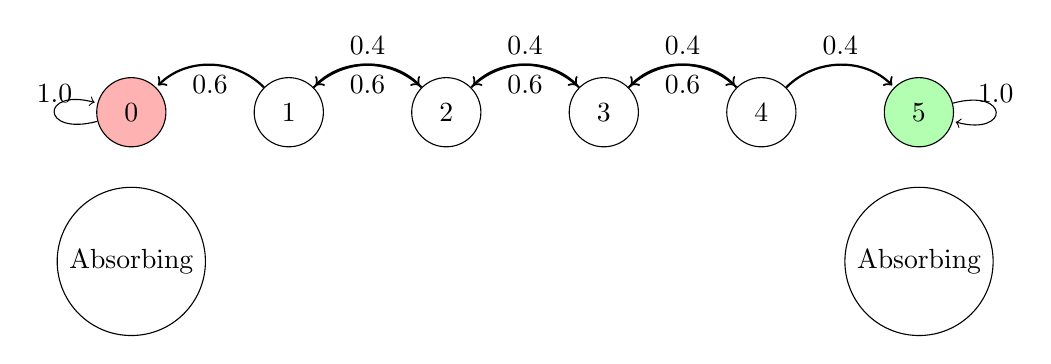
\begin{tikzpicture}[shorten >=1pt, node distance=2cm, auto, scale=1.5]

        % Nodes representing the states
        \node[state, fill=red!30] (A) {0};
        \node[state, right of=A] (B) {1};
        \node[state, right of=B] (C) {2};
        \node[state, right of=C] (D) {3};
        \node[state, right of=D] (E) {4};
        \node[state, fill=green!30, right of=E] (F) {5};
    
          % Transitions between states with different arrow types
    \path[->, thick] (B) edge [bend left=45, above] node {0.4} (C);
    \path[->, thick] (B) edge [bend right=45, below] node {0.6} (A);
    \path[->, thick] (C) edge [bend left=45, above] node {0.4} (D);
    \path[->, thick] (C) edge [bend right=45, below] node {0.6} (B);
    \path[->, thick] (D) edge [bend left=45, above] node {0.4} (E);
    \path[->, thick] (D) edge [bend right=45, below] node {0.6} (C);
    \path[->, thick] (E) edge [bend left=45, above] node {0.4} (F);
    \path[->, thick] (E) edge [bend right=45, below] node {0.6} (D);
    
    
        % Absorbing states
        \node[draw, circle, below=0.5cm of A] (AbsA) {Absorbing};
        \node[draw, circle, below=0.5cm of F] (AbsF) {Absorbing};
        
        % Final connections
        \path[->] (A) edge [loop left, above] node {1.0} (A);
        \path[->] (F) edge [loop right, above] node {1.0} (F);
    \end{tikzpicture}
    
    The process \( X_n \) is a Markov chain because the probability of transitioning to the next state depends only on the amount of wealth at the current state, not on the history of previous states. The Markov property holds because the future state depends only on the current state, making it a memoryless process.
    
    \item[(b)] \textbf{(4 points)} Construct the transition probability matrix for the Markov chain, ensuring that it captures both the winning and losing probabilities. Explicitly show the entries corresponding to the absorbing states and transient states.
\[
P =
\begin{array}{c|cccccc}
\text{State} & 0   & 1   & 2   & 3   & 4   & 5   \\
\hline
0 & 1   & 0   & 0   & 0   & 0   & 0   \\
1 & 0.6 & 0   & 0.4 & 0   & 0   & 0   \\
2 & 0   & 0.6 & 0   & 0.4 & 0   & 0   \\
3 & 0   & 0   & 0.6 & 0   & 0.4 & 0   \\
4 & 0   & 0   & 0   & 0.6 & 0   & 0.4 \\
5 & 0   & 0   & 0   & 0   & 0   & 1   \\
\end{array}
\]    
\item[(c)] \textbf{(5 points)} Derive the probability that the gambler reaches the absorbing state at \( N = 5 \) dollars before reaching 0 dollars (ruin).
    \\ let \( P \) be the probability of reaching the absorbing state at \( N = 5 \) dollars before reaching 0 dollars (ruin) given the current wealth of the gambler is \( i \), where \( i \) is the current state of the Markov chain. The probability \( P \) can be expressed as:
    \[
    P = \begin{cases}
    1, & \text{if } i = 5, \\
    0, & \text{if } i = 0, \\
    0.6P_{i-1} + 0.4P_{i+1}, & \text{otherwise}.
    \end{cases}
    \]
    The probability \( P \) can be solved using the system of linear equations:
    \[
    \begin{aligned}
    P_0 & = 0, \\
    P_5 & = 1, \\
    P_1 & = 0.6P_0 + 0.4P_2, \\
    P_2 & = 0.6P_1 + 0.4P_3, \\
    P_3 & = 0.6P_2 + 0.4P_4, \\
    P_4 & = 0.6P_3 + 0.4P_5.
    \end{aligned}
    \]
    Solving the system of equations, we find that the probability \( P \) is:
    \[
    P = \begin{cases}
    0, & \text{if } i = 0, \\
    \frac{1}{5}, & \text{if } i = 1, 2, 3, 4, \\
    1, & \text{if } i = 5.
    \end{cases}
    \]
    Therefore, the probability that the gambler reaches the absorbing state at \( N = 5 \) dollars before reaching 0 dollars (ruin) is \( \frac{1}{5} \) for all states \( i = 1, 2, 3, 4 \).

    \item[(d)] \textbf{(3 points)} Discuss how the probabilities change as \( p \) varies, particularly focusing on the expected duration of the game and the likelihood of reaching 5 dollars versus 0 dollars.
    \\\\ The probability of reaching the absorbing state at \( N = 5 \) dollars before reaching 0 dollars (ruin) depends on the winning probability \( p \). As \( p \) increases, the gambler is more likely to reach 5 dollars before reaching 0 dollars. The expected duration of the game decreases as \( p \) increases, as the gambler is more likely to win and reach the target wealth of 5 dollars. Conversely, as \( p \) decreases, the gambler is more likely to lose and reach 0 dollars, leading to a longer duration of the game.
    \item[(e)] \textbf{(10 points)} Simulate a gambling game where you either win or lose money based on specific probabilities based on the above parameters. 




\subsection*{Simulation Steps}

\begin{enumerate}
    
    \item \textbf{Initialize Simulation:}
    \begin{itemize}
        \item Define the number of trials (\texttt{num\_trials = 10}) to run, starting wealth for the player, probability of winning each round, and the target wealth to reach.
    \end{itemize}
    
    \item \textbf{Conduct Trials:}
    \begin{itemize}
        \item For each trial:
        \begin{itemize}
            \item Start with the initial wealth.
            \item Track the wealth changes throughout the game.
            \item Simulate rounds of play:
            \begin{itemize}
                \item Continue playing until either the target wealth is reached or the player loses all their money.
                \item In each round, determine the outcome based on the defined probability, updating the wealth accordingly.
            \end{itemize}
        \end{itemize}
    \end{itemize}
    
    \item \textbf{Store Results:}
    \begin{itemize}
        \item Keep a record of the wealth progression for each trial.
    \end{itemize}
    
    \item \textbf{Visualize Outcomes:}
    \begin{itemize}
        \item Create plots to illustrate the wealth changes over the course of several trials.
        \item Mark significant states, such as the target wealth and the point of ruin.
    \end{itemize}
    
    \item \textbf{Analyze Results:}
    \begin{itemize}
        \item Calculate the number of times the player wins or loses across all trials.
        \item Determine the overall winning rate and the average number of rounds played per trial.
        \item Present these statistics for review.
    \end{itemize}
\end{enumerate}

\subsection*{Discussion Points}
\begin{itemize}
    \item Reflect on how the probabilities affect the game's dynamics.
    \item Consider the implications of reaching either absorbing state and the significance of randomness in this process.
    \item Discuss how this simulation relates to concepts of Markov chains and random walks.
\end{itemize}


\end{itemize}




\end{document}